\documentclass{beamer}
% \usepackage{animate}
\usepackage{multimedia}
\usepackage[english,russian]{babel}

\usepackage{pgfpages}
\setbeameroption{show notes on second screen}
%https://tug.ctan.org/macros/latex/contrib/beamer/doc/beameruserguide.pdf

\usepackage[T2A]{fontenc}
\usepackage[utf8]{inputenc}

\setbeamertemplate{caption}[numbered]

\usetheme{CambridgeUS}
\usecolortheme{dolphin}


\title[Модель Блинна-Фонга]{Модель освещения Блинна-Фонга}
\author[Быковских Д.А.]{Быковских Дмитрий Александрович}
\date{30.11.2024}

\begin{document}
	\begin{frame}
		\titlepage
	\end{frame}

	\begin{frame}{Введение}
		Модель освещения Фонга является простой, популярной и широко известной в компьютерной графике.

		Описание модели было представлено в следующей статье

		\href{https://users.cs.northwestern.edu/~ago820/cs395/Papers/Phong_1975.pdf}{Bui Tuong Phong  
		"Illumination for Computer Generated Pictures"~
		University of Utah (1975 г.)}

		\note{
			\begin{figure} 
				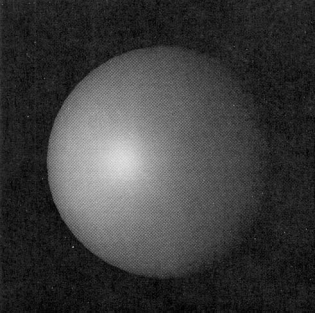
\includegraphics[width=0.45\textwidth]{images/modeled-sphere.png}
				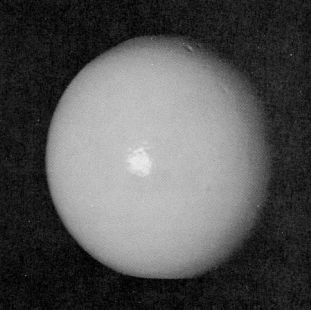
\includegraphics[width=0.45\textwidth]{images/real-sphere.png}
			\caption{Изображения из статьи: сфера, отображенная с улучшенным затенением (слева); фотография реальной сферы(справа)}
		\end{figure}
		}
		
	\end{frame}

	\begin{frame}{Введение}
		В основе модели освещения Фонга лежит алгоритм приближенного расчета интенсивности света на поверхности объектов. 

		Один из вариантов рабочей формулы имеет вид:

		\[
			I = I_a k_a + \sum_{j=1}^{m} \frac{I_{j}}{d+k} \bigg[ k_d (N_j \cdot L_j) + k_s (R_j \cdot V)^{\alpha_j} \bigg]
		% ,
		\]

		\begin{figure} 
			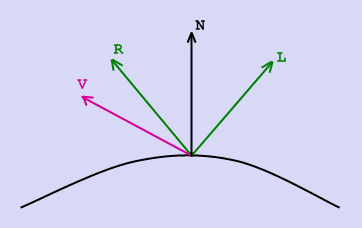
\includegraphics[width=0.45\textwidth]{images/specular_light.png}
			\caption{Схема расположения векторов модели освещения}
		\end{figure}


		\note{
			Формула состоит из следующих частей:
			\begin{itemize}
				\item фоновое освещение $I_a$;
				\item количество ИС $m$;
				\item интенсивность излучения $j$-го источника света $I_j$;
				\item функция затухания $\frac{1}{d+k}$;
				\item свойства поверхности $k_a, k_d, k_s$ в точке поверхности;
				\item диффузное рассеивание $(N_j \cdot L_j)$;
				\item зеркальное рассеивание $(R_j \cdot V)^{\alpha_j}$.
			\end{itemize}

			Настройка этих компонентов позволяет создавать реалистичные изображения (для того времени) трехмерных объектов с учетом их взаимодействия с источниками света. 
		}

	\end{frame}

	\if 0
	\begin{frame}{Источники света (ИС)}
		ИС (Light)~---~любой объект, излучающий энергию. \\
		Типы источников света:
		\begin{itemize}
			\item Источники направленного света;
			\item Точечные ИС;
			\item Прожекторы.
		\end{itemize}
		% \[
		% \begin{pmatrix}
		% 	Параметры
		% \end{pmatrix}	
		% \]
		\note{
			% \begin{figure} 
			% 	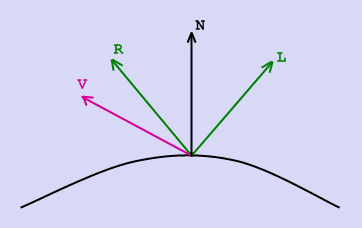
\includegraphics[width=0.75\textwidth]{images/specular_light.png}
			% 	\caption{Схема расположения векторов модели освещения}
			% \end{figure}
		}

	\end{frame}
	\fi

	\begin{frame}{Источники света (ИС) и интенсивность излучения}

		ИС (Light)~---~любой объект, излучающий энергию. 

		Интенсивность излучения ($I$)~---~физическая величина, характеризующая мощность электромагнитного излучения (например, света) в определенном направлении от источника. 
		
		\vspace{1cm}

		Математически интенсивность излучения рассчитывается как:
		\[
			I= \frac{P}{A}
			,
		\]
		где
    % $I$~---~интенсивность излучения,
    $P$~---~мощность излучения (в ваттах),
    $A$~---~площадь, через которую проходит излучение (в м$^2$).
		
		
		\note{
			Следует понимать, что:	
		
			1. Значения Для каждой компоненты цвета считается независимо, т.е. $I = (I_r, I_g, I_b)$.
			
			2. Суммарное освещение вычисляется как:
			\[
				I = k_e + k_a I_{a} + \sum_j I_j
			,
			\]
			где 
			$k_e$~---~коэффициент излучения светом материалом;\\
			$k_a I_{a}$~---~глобальная фоновая освещенность сцены;\\
			$I_j$~---~вклад вносимый $j$-м ИС.
			}

	\end{frame}

	\begin{frame}{Радиальное затухание}

		Известно, что чем дальше расположен объект от ИС, тем слабее интенсивность света на поверхности этого объекта.\\
		Поэтому необходимо учитывать интенсивность затухания (attenuation) света между источником света и поверхностью.

		\vspace{.2cm}		
		Интенсивность радиального затухания света определяется законом обратных квадратов (Inverse-Square Law):
		\[
			f_r(d) \sim \frac{1}{d^2}
			,
		\]
		где $d$~---~расстояние от объекта до ИС.
		
		% \vspace{.15cm}		
		Но на практике применяют следующую функцию
			
		\[
			f(d) = 
			\begin{cases}
				\frac{1}{a_0+a_1 d + a_2 d^2}, \quad \text{для локальных ИС} \\	
				1, \quad \text{для бесконечно-удаленных ИС} \\	
			\end{cases}	
			,
		\]
		где $a_0, a_1, a_2$~---~коэффициенты, подбираемые практическим путем в зависимости от сцены.

		\note{
			\begin{figure} 
				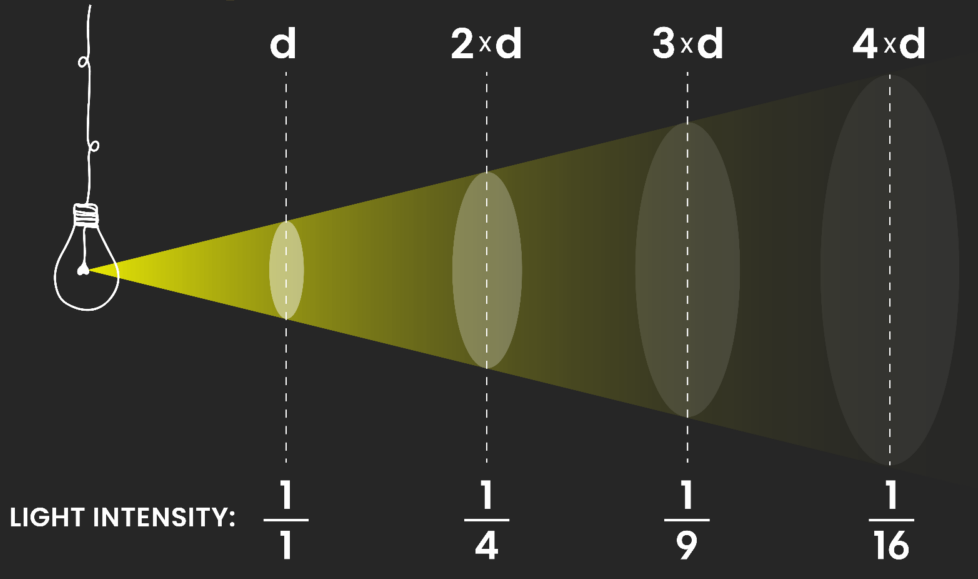
\includegraphics[width=0.85\textwidth]{images/inverse-square-law.png}
			\caption{\href{https://progradedigital.com/understanding-and-using-the-inverse-square-law-in-photography/}{Закон обратных квадратов}}
		\end{figure}
		}

	\end{frame}

	\begin{frame}{Угловое затухание}
		% Амплитуда затухания определяется функцией углового затухания.\\
		Угловое затухание~---~явление, при котором интенсивность света затухает по мере увеличения угла между направлением, из которого свет падает, и нормалью к поверхности. 
		% Это явление учитывается в моделях освещения для того, чтобы объекты визуально выглядели естественно, с учетом изменения интенсивности света в зависимости от угла падения.

		%Математически угловое затухание интенсивности часто выражается с использованием косинуса угла между направлением света и нормалью к поверхности. 
		% Если $\theta$~---~угол между направлением света и нормалью в точки поверхности, то угловое затухание может быть выражено следующим образом:

		Угловое затухание интенсивности выражается следующей формулой
		\[
			f_{\alpha}(\theta) = \cos^{\alpha} \theta
			=
			\bigg( \frac{L \cdot D}{ \lvert L \rvert \lvert D \rvert} \bigg)^\alpha
		\]
		% \[
		% 	f_{\alpha}(\theta) 
		% 	=
		% 	\max(0, (\cos\theta)^\alpha)
		% 	= 
		% 	\max\Bigg(0, \bigg( \frac{L \cdot D}{ \lvert L \rvert \lvert D \rvert} \bigg) ^\alpha \Bigg)
		% 	,
		% \]
		где
		$L$~---~вектор направления от источника света к точке поверхности освещения;
		$D$~---~вектор направления источника света;
		$\theta$~---~угол между этими векторами;
		$\alpha$~---~коэффициент фокусировки, управляющий концентрацией света внутри конуса.


		\footnotesize
		Примечание.\\
		Коэффициент углового затухания $\theta$ уменьшает интенсивность света по мере увеличения угла. 
		Когда свет падает под прямым углом (угол), угловое затухание равно 1, и свет не затухает. 
		При увеличении угла, значение косинуса уменьшается, что приводит к уменьшению интенсивности света.

		При $\alpha << 1$ получается имитация мягкого, рассеянного света.\\
		При $\alpha >> 1$ ---  имитация узкого прожектора или лазера.

		\note{
			\begin{figure} 
				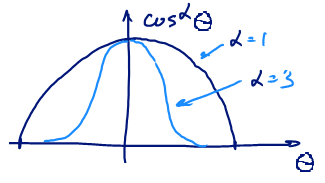
\includegraphics[width=0.85\textwidth]{images/Angular-intensity-attenuation.png}
				\caption{Интенсивность затухания света в зависимости от угла $\theta$ 
				%(т.е. между обратным вектором направления света к объекту и нормалью к точки поверхности) 
				и коэффициента фокусировки $\alpha$}
			\end{figure}
		}
		
	\end{frame}


	\begin{frame}{Источники направленного света}
		Направленный ИС (Directional Light).\\
		Лучи света расположены параллельны друг другу и движутся в определенном направлении. \\
		
		\[
			I_{\text{dir}} 
			= 
			I_0 \cdot \max \bigg( 0, \frac{(L \cdot N)}{\lvert L \rvert \lvert N \rvert} \bigg)
			= 
			I_0 \cdot \max(0,  \cos \phi)
			,
		\]
		где
		
		$I_0$~---~начальная интенсивность направленного источника света.

		$L$~---~вектор направления света;

		$N$~---~вектор нормали поверхности;
		
		$\phi$~---~угол между этими векторами.


		Применение:
		
		Этот ИС моделируют бесконечно удаленный источник света, такой как солнце. 

		Они используются для создания резких теней и подчеркивания форм объектов.

		\note{
			\begin{figure} 
				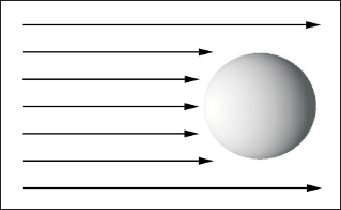
\includegraphics[width=0.75\textwidth]{images/f05_05.jpg}
				\caption{Источник направленного света}
			\end{figure}
		}
		
	\end{frame}
	
	\begin{frame}{Точечные ИС}
		Точечный ИС (Point Light)
		расположен в конкретной точке пространства и светит равномерно во всех направлениях.

		\[
			I_{\text{point}} = I_0 \cdot f_r(d) \cdot 
			\max \bigg( 0, \frac{(L \cdot N)}{\lvert L \rvert \lvert N \rvert} \bigg)
			,
		\]
		где $d$~---~расстояние от точечного источника света до освещаемой точки.

		Применение:

		Имитация искусственного освещения, например, лампочки или фонари. 
		
		Общее освещение в сценах с несколькими точечными источниками для создания объемного света.

		Моделирование огоньков или звезд в реалистичных или стилизованных сценах.

		\note{
			\begin{figure} 
				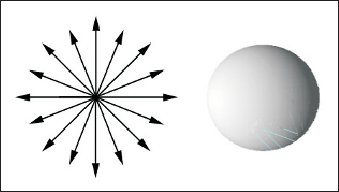
\includegraphics[width=0.85\textwidth]{images/f05_04.jpg}
			\caption{Точечный ИС}
		\end{figure}
		}
	\end{frame}


	
	\begin{frame}{Споты и прожекторы}
		Спот (Spot Light) или прожектор (Projector). \\
		
		Является частным случаем точечного источника, но свет от него распространяется только внутри ограничивающего конуса, а не по всем направлениям.
		% Этот ИС создает конус света, направленный в определенном направлении.\\

		% Используются для создание направленного света в определенных направлениях.
		% Также могут быть применяться для проецирования текстур или изображений на поверхности объектов в сцене. 

				% \[
		% 	f(\phi) 
		% 	= 
		% 	\bigg[ \frac{(v_o, v_l)}{|v_o||v_l|} \bigg]^{a_l}
		% 	=
		% 	\text{cos} ^{a_l} \phi
		% 	,
		% \]

		\[
			I_{\text{point}} = I_0 \cdot f_r(d) \cdot f^*_{\alpha}(\theta) \cdot 
			\max \bigg( 0, \frac{(L \cdot N)}{\lvert L \rvert \lvert N \rvert} \bigg)
			,
		\]
		где 
		$
			f^*_a(\theta) = \begin{cases} 
			\cos^{\alpha} \theta, & \text{если } \cos \theta > \cos \theta_{\text{outer}} \\
			0, & \text{если } \cos \theta \leq \cos \theta_{\text{outer}}
			\end{cases}
			,
		$ 
		где 
		$0 \le \theta \le \theta_{\text{outer}}$.

		Применение:

		Такой тип ИС эффективен для выделения конкретных объектов или областей в сцене.
		
		Точечный ИС может имитировать направленные лучи фар автомобилей или прожекторы на сцене.

		\note{
			\begin{figure} 
				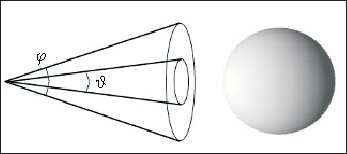
\includegraphics[width=\textwidth]{images/f05_06.jpg}
			\caption{Прожекторы}
		\end{figure}
		}
	\end{frame}


	\if 0

	\begin{frame}{Эффекты освещения поверхности}
		\begin{figure} 
			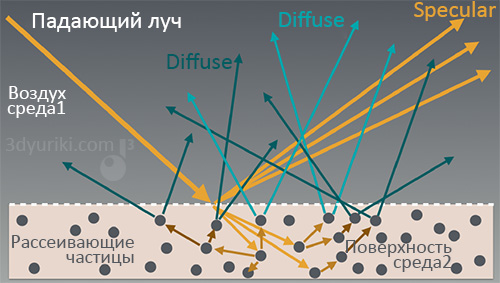
\includegraphics[width=0.8\textwidth]{images/4-kak-proishodit-rasseivanie-sveta-v-materiale.jpg}
			\caption{Рассеивание света в материале}
		\end{figure}
		
		% Вот несколько основных эффектов освещения поверхности:

		% \begin{itemize}
		% 	\item Фоновое освещение (Ambient Occlusion, $k_a$);
		% 	\item Рассеянное освещение (Diffuse Lighting, $k_d$);
		% 	\item Зеркальное отражение (Specular Reflection, $k_s$);
		% 	\item Отраженный свет (Reflection);
		% 	\item Преломление (Refraction);
		% 	\item Тени (Shadows);
		% 	\item Глосс (Gloss).
		% \end{itemize}
		
		\note{
			\scriptsize
		
			В компьютерной графике эффекты освещения поверхности важны для создания реалистичных и привлекательных визуальных изображений. Эти эффекты обусловлены взаимодействием света с материалами поверхности объектов. 

			Ambient Occlusion (AO) моделирует затемнение в областях, где свет имеет ограниченный доступ. Он усиливает визуальное восприятие объемности объектов, подчеркивая скрытые участки.

			Рассеянное освещение (Diffuse Lighting) характеризуется равномерным рассеиванием света в различных направлениях на поверхности объекта. Интенсивность рассеянного света зависит от угла между направлением света и нормалью к поверхности. Материалы с рассеянным освещением выглядят матовыми.

			Зеркальное отражение (Specular Reflection) связан с отражением света в направлении, симметричном относительно зрителя. Зеркальное отражение создает блики на поверхности материала и придает объекту блеск. Эффект сильнее выражен у гладких и блестящих материалов.
			
			Преломление (Refraction) происходит, когда свет проходит через прозрачные материалы. Этот эффект приводит к изменению направления света и созданию искажений на границе между материалами с разными оптическими свойствами.
	
			Тени (Shadows) создаются благодаря препятствиям, которые мешают свету достигнуть определенных областей поверхности. Тени важны для добавления глубины и реализма в изображения.

			Отраженный свет (Reflection) моделирует отражение окружающей среды на поверхности объекта. Это может включать отражение других объектов, окружения или облаков.
	
			%Глосс (Gloss). Этот эффект описывает степень блеска или матовости поверхности. Гладкие и блестящие поверхности имеют низкую степень матовости, в то время как матовые материалы выглядят более матовыми.
			
		}
	\end{frame}
	\fi

	\begin{frame}{Свойства материала}
		Когда речь идет о свойствах материала в приложении к освещению, то имеется в виду его способность воспринимать каждую из трех компонент света каждой составляющей освещенности: \\
		$k_a$~---~свойство материала воспринимать фоновое освещение; \\
		$k_d$~---~свойство материала воспринимать рассеянное освещение; \\
		$k_s$~---~свойство материала воспринимать зеркальное освещение.
		% Т.о. цветовые свойства материала задаются коэффициентами, которые объединяются в тройки. \\
		
		\vspace{0.3cm}
		Дополнительно, к свойствам материала добавляются еще коэффициенты: \\
		$k_e$~---~свойство материала излучать свет; \\
		% $k_{\alpha}$~---~прозрачность; \\
		$\alpha$~---~коэффициент блеска. 
		
		\note{

			\begin{figure} 
				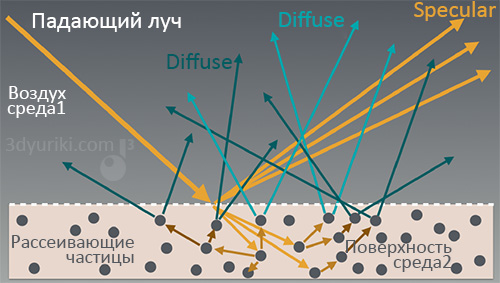
\includegraphics[width=0.9\textwidth]{images/4-kak-proishodit-rasseivanie-sveta-v-materiale.jpg}
				\caption{Рассеивание света в материале}
			\end{figure}
		}
	\end{frame}




	\begin{frame}{Вычисление угла между отраженным лучом и направлением на наблюдателя}
		Угол между отраженным лучом и направлением на наблюдателя можно рассчитать по следующей формуле:

		\[
			R + L=2(N \cdot L) N	
		\]
		\[
			R = 2 (N \cdot L) N - L
		\]

		Скалярное произведение $(R \cdot V)$ рассчитывается по формуле:

		\[
			(R \cdot V) =2({N}\cdot{L})({N}\cdot{V})-({L}\cdot{V})
		\]

		\footnotesize
		Примечание.\\
		Формула проекции вектора $L$ на вектор $N$
		\[
			\text{Proj}_{N} L = \frac{(L \cdot N)}{\lvert N \rvert} N
		\]


		\note{
			\begin{figure} 
				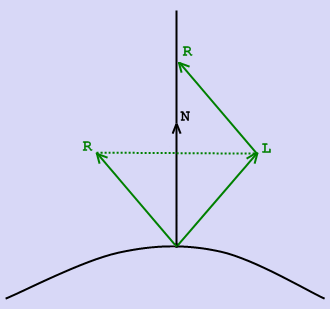
\includegraphics[width=0.5\textwidth]{images/reflect_vector.png}
			\caption{Векторы в модели освещенности Блинна}
		\end{figure}

		}

	\end{frame}




	\begin{frame}{Фоновое освещение}

		Часто просто задается некое глобальное фоновое освещение всей сцены, которое можно выразить с помощью некоторой формулы

		\[
			I = k_a I_a
			,
		\]
		где 
		
		$I_a$~---~фоновая составляющая освещенности в точке;

		$k_a$~---~коэффициент фонового освещения (свойство материала воспринимать фоновое освещение);
		
		$I$~---~интенсивность фонового освещения.
		
		\footnotesize
		Примечание.\\
		Фоновая составляющая освещенности не зависит от пространственных координат освещаемой точки и источника. 
		Поэтому при моделировании освещения, в большинстве случае, не имеет смысла брать более одного фонового источника света. 
		
		
		\note{
			\begin{figure} 
				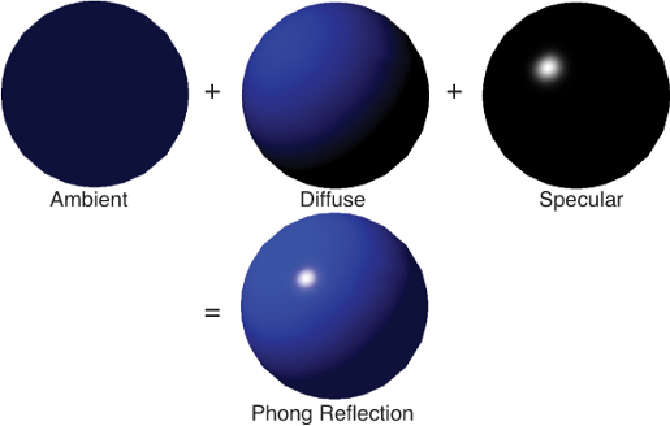
\includegraphics[width=0.8\textwidth]{images/img-gen171.png}
				\caption{Виды отражений в модели освещения Фонга}
			\end{figure}
		}
	\end{frame}

	\begin{frame}{Рассеянный свет}	

		Рассеянное освещение (Diffuse Reflection)
		
		описывает равномерное рассеивание света от поверхности во всех направлениях.

		Расчетная формула имеет следующий вид:
		
		\[
			I_d %= k_d \cos (L \cdot N) I_d 
			= k_d (L \cdot N) I_d
			,	
		\]
		где 
		$I_d$~---~рассеянная составляющая освещенности в точке;
		$k_d$~---~свойство материала воспринимать рассеянное освещение;
		$I_d$~---~мощность рассеянного освещения;
		$L$~---~направление из точки на источник;
		$N$~---~вектор нормали в точке.
	
		\footnotesize
		Примечание.\\ 
		Интенсивность рассеянного света зависит от угла между нормалью к поверхности и направлением света.
		
		\note{
			\begin{figure} 
				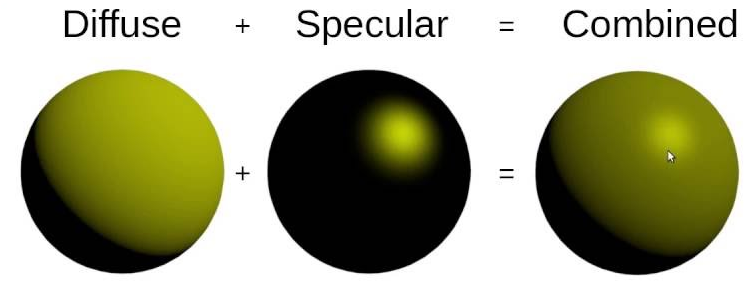
\includegraphics[width=1.0\textwidth]{images/diffuse_specular.png}
				\caption{Виды отражений без учета фонового освещения в модели освещения Фонга}
			\end{figure}
		}

	\end{frame}

	% \begin{frame}{Рассеянное освещение}
	% 	Рассеянное освещение~---~это один из компонентов модели освещения, используемый для приближенного моделирования того, как свет рассеивается на матовых поверхностях. Оно описывает явление равномерного рассеивания света во всех направлениях от поверхности.

	% 	Основная идея рассеянного освещения заключается в том, что поверхность, на которую падает свет, диффузно рассеивает его во все стороны. Интенсивность рассеянного света зависит от угла между направлением падающего света и нормалью к поверхности в данной точке. Чем ближе угол к 90 градусам (то есть, чем более свет падает под прямым углом к поверхности), тем интенсивнее рассеянный свет.
		
	% 	Математически это часто выражается с использованием закона Ламберта. Если NN - нормализованный вектор нормали к поверхности, LL - нормализованный вектор направления света, и IdId - интенсивность диффузного освещения, то интенсивность рассеянного света (IdiffuseIdiffuse) может быть выражена следующим образом:
		
	% 	\[
	% 		Idiffuse=Id \cdot (N \cdot L)Idiffuse = Id \cdot (N\cdot L)
	% 	\]
		
	% 	Здесь обозначает скалярное произведение векторов.
		
	% 	Рассеянное освещение вместе с другими компонентами, такими как зеркальное отражение и затухание, формирует комплексные модели освещения, используемые в компьютерной графике для создания более реалистичных изображений трехмерных сцен.
	% \end{frame}

	\begin{frame}{Зеркальное отражение}

		Зеркальное отражение (Specular Reflection) 
		
		моделирует отражение света от блестящих или гладких поверхностей. 

		Этот компонент создает яркие блики на поверхности и зависит от угла между направлением обзора (направление, с которого наблюдается поверхность) и направлением отраженного света.

		\[
			I_s = k_s \cos^{\alpha}(R,V) I_s = k_s (R \cdot V)^{\alpha} I_s
			,	
		\]
		где
		$I_s$~---~зеркальная составляющая освещенности в точке;
		$k_s$~---~коэффициент зеркального отражения;
		$I_d$~---~мощность зеркального освещения;
		$R$~---~направление отраженного луча;
		$V$~---~направление на наблюдателя;
		$\alpha$~---~коэффициент блеска, свойство материала.


		\note{
			Именно зеркальное отражение представляет наибольший интерес, но в то же время его расчет требует больших вычислительных затрат. При фиксированном положении поверхности относительно источников света фоновая и рассеянные составляющие освещения могут быть просчитаны единожды для всей сцены, т.к. их значение не зависит от направления взгляда. С зеркальной составляющей этот фокус не сработает и придется пересчитывать её каждый раз, когда взгляд меняет свое направление.

			Во всех вычислениях выше, для рассеянной и зеркальной компонент, если скалярное произведение в правой части меньше нуля, то соответствующая компонента освещенности полагается равной нулю.
		}
	\end{frame}

% 	\begin{frame}{Зеркальное отражение}
% 		Зеркальное освещение~---~это компонент модели освещения, который моделирует отражение света от блестящих или гладких поверхностей. Этот компонент отвечает за появление на поверхности ярких бликов, которые образуются при отражении света в определенном направлении.

% Основные характеристики зеркального отражения включают в себя:

%     Отражательный вектор (Reflectance Vector): Он представляет собой направление, в котором свет отражается от поверхности. Для вычисления отражательного вектора используется зеркальное отражение относительно нормали к поверхности.

%     Блеск (Specular Highlight): Это яркое пятно на поверхности, которое возникает в результате зеркального отражения света. Чем ближе угол между направлением обзора (точка, с которой мы смотрим на объект) и отражательным вектором к 0 градусам, тем более ярким будет блеск.

% 		Математически зеркальное отражение часто описывается с использованием модели Фонга или модели Блинна-Фонга. Для данной точки на поверхности с нормалью NN, вектором направления света LL, вектором обзора VV и коэффициентом блеска ksks, интенсивность зеркального отражения (IspecularIspecular) может быть выражена следующим образом:

% 		\[
% 			Ispecular=ks \cdot (R \cdot V)nIspecular=ks\cdot (R\cdot V)n
% 		\]

% 		где RR - отражательный вектор, VV - вектор обзора, и nn - экспоненциальный коэффициент, который определяет степень блеска.

% 		Зеркальное освещение вместе с другими компонентами, такими как рассеянное освещение и затухание, входит в состав моделей освещения, используемых в компьютерной графике для достижения более реалистичных эффектов.
% 	\end{frame}


	\begin{frame}{Модель освещения и методы затенения}
		\[
			I = k_e + I_a k_a + \sum_{j=1}^{m} \frac{I_{j}}{d+k} \bigg[ k_d (N_j \cdot L_j) + k_s (R_j \cdot V)^\alpha \bigg]
		,
		\]

		\footnotesize
		где
		$I$~---~интенсивность излучения;
		$k_e$~---~способность материала излучать свет;
		$I_a$~---~интенсивность фонового излучения;
		$k_a$~---~коэффициент фонового отражения;
		$I_j$~---~интенсивность ИС;
		$d$~---~расстояние от ИС до объекта;
		$k$~---~константана (трюк, чем ближе, тем больше величина);
		$k_d$~---~коэффициент диффузного отражения;
		$k_s$~---~коэффициент зеркального отражения;
		$\alpha$~---~коэффициент блеска поверхности материала;
		$N_j$~---~нормаль в точке поверхности;
		$L_j$~---~вектор направления на ИС;
		$R_j$~---~вектор отражения ИС;
		$V$~---~вектор направления камеры или точки обзора;
		$m$~---~количество ИС.

		\vspace{0.15cm}
		Сравнение простейших методов затенения.

		В методе плоского затенения освещение вычисляется один раз для каждого полигона в сцене.

		В методе затенения по Фонгу для каждой вершины полигона вычисляются значения нормали и освещенности. Затем значения этих характеристик интерполируются между вершинами, чтобы получить плавное изменение освещенности на всей поверхности полигона.



		
		\note{
			\begin{figure} 
				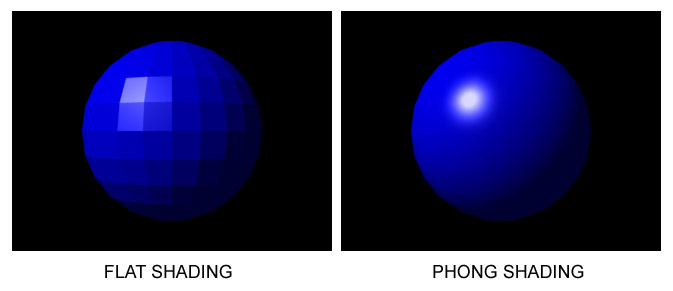
\includegraphics[width=\textwidth]{images/7UNuF.jpg}
			\caption{Сравнение затенений: плоское (слева); по Фонгу (справа)}
		\end{figure}
		}
	\end{frame}


	\begin{frame}{Модель освещения Блинна-Фонга}{Упрощенный расчет зеркальной компоненты освещенности}
		
		Модель освещения Блинна-Фонга (1977 г.) представляет собой модель освещения Фонга с упрощенным расчетом зеркального отражения. 
		Это позволяет сэкономить вычислительные ресурсы, что было важно даже для такой простой модели освещения.\\
		Вычисление в каждой точке поверхности вектора полупути $H$ (halfway vector) выполняется по следующей формуле:
		\[
			H=\frac{L+V}{|L+V|}
			,
		\]
		который показывает ориентацию площадки, на которой будет максимальное отражение. 
		\\
		Тогда величину $(R\cdot V)^\alpha$ можно заменить величиной $(H \cdot N)^{\alpha}$.

		% При этом α <> β и, в общем случае, соотношение между ними зависит от пространственной связи векторов {V}, {L} и {N}. Вектор {H} называется вектором полупути, т.к. если все три вектора {V}, {L} и {N} лежат в одной плоскости, то угол между {H} и {N} составляет половину угла между {R} и {V}.

		% Модель отражения Блинна-Фонга никогда в точности не совпадает с моделью Фонга, однако можно подобрать соответствующие значения α и β, для которых распределения зеркальной составляющей по поверхности для обеих моделей будут очень близкими. Вместе с тем, в ряде случаев модель Блинна-Фонга требует значительно меньше вычислений, например в случае направленного бесконечно-удаленного источника.

		\note{
			\begin{figure} 
				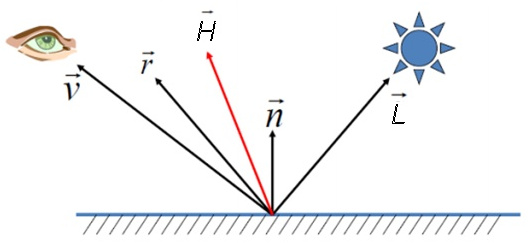
\includegraphics[width=1.0\textwidth]{images/physics_vector_blinna_fonga.jpg}
				\caption{Векторы в модели освещения Блинна-Фонга}
			\end{figure}
			}
	\end{frame}

	\begin{frame}{Модель освещения Блинна-Фонга}
		\[
			I = k_e + I_a k_a + \sum_{j=1}^{m} \frac{I_{j}}{d+k} \bigg[ k_d (N_j \cdot L_j) + k_s (N_j \cdot H)^{\alpha_j} \bigg]
		,
		\]
		где
		$I$~---~интенсивность излучения;
		$k_e$~---~способность материала излучать свет;
		$I_a$~---~интенсивность фонового излучения;
		$k_a$~---~коэффициент фонового отражения;
		$I_j$~---~интенсивность ИС;
		$d$~---~расстояние от ИС до объекта;
		$k$~---~константана (трюк, чем ближе, тем больше величина);
		$k_d$~---~коэффициент диффузного отражения;
		$k_s$~---~коэффициент зеркального отражения;
		$\alpha$~---~коэффициент блеска поверхности материала;
		$N_j$~---~нормаль в точке поверхности;
		$L_j$~---~вектор направления на ИС;
		$H$~---~вектор полупути (halfway vector);
		$V$~---~вектор направления камеры или точки обзора;
		$m$~---~количество ИС.

		\note{
			\begin{figure} 
				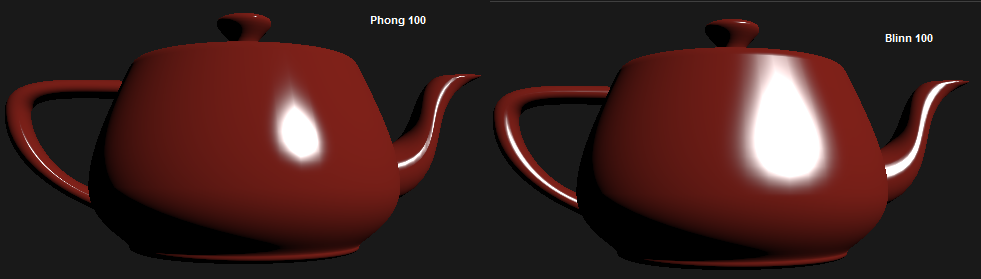
\includegraphics[width=\textwidth]{images/phong-blinn-compare.png}
			\caption{Сравнение моделей Фонга и Блинна-Фонга}
		\end{figure}
		}

	\end{frame}

	% \begin{frame}{Заключение}
	% 	Литература
	% 	\begin{enumerate}
	% 		\item \href{https://users.cs.northwestern.edu/~ago820/cs395/Papers/Phong_1975.pdf}{Bui Tuong Phong  
	% 		"Illumination for Computer Generated Pictures"~
	% 		University of Utah (1975 г.)}
	% 		\item \href{}{}
	% 	\end{enumerate}
	% \end{frame}

\end{document}
